% ============================================================================
% Figure 4: Encoding complexity versus observed outcome (descriptive, no correlation claimed).
% Data source: clause counts computed exactly from src/sudoku/solvers/sat.py
% formulas (groups = 4N^2; per-encoding AMO clauses + one ALO per group + clue units).
% Outcome counts from data/results/benchmark_sat_vs_nonsat.csv (SAT only, 7 configs).
% Panel A: total clauses vs N (log y) for each AMO encoding at N in {9,36,81};
% pairwise and binary at N=81 are marked EXCLUDED (memory guard, ~85M clauses).
% Panel B: stacked outcome counts per stratum (SAT pooled, 7 configs):
% valid vs timeout vs predeclared-excluded vs live-guard-rejection.
% NOTE: runtimes are successful-run-only and timeout-censored; no statistical
% correlation between clause count and runtime has been analyzed.
% ============================================================================
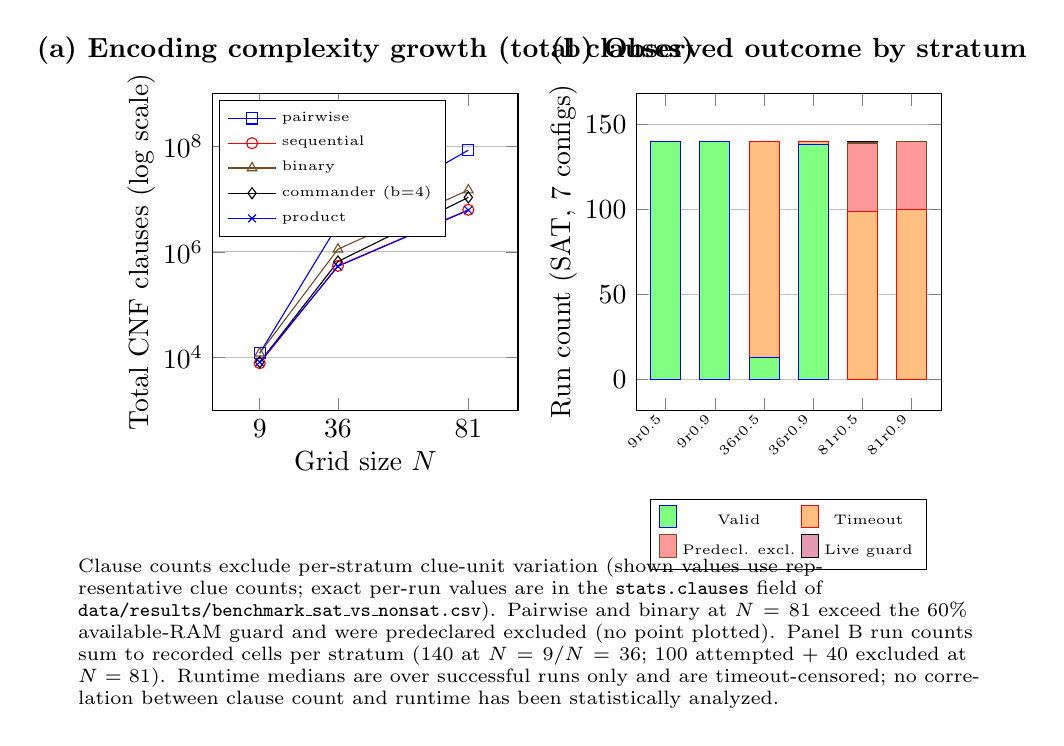
\begin{tikzpicture}
  % ---- Panel A: clause count growth vs N (log scale) ----
  \begin{axis}[
    name=plotA,
    ymode=log,
    ymin=1e3, ymax=1e9,
    xmin=5, xmax=86,
    xtick={9,36,81},
    xlabel={Grid size \(N\)},
    ylabel={Total CNF clauses (log scale)},
    ylabel style={yshift=-0.4em},
    xlabel style={yshift=0.2em},
    ymajorgrids=true,
    title style={font=\bfseries, yshift=0.1em},
    title={(a) Encoding complexity growth (total clauses)},
    width=0.45\textwidth, height=5.6cm,
    legend style={at={(0.02,0.98)}, anchor=north west, font=\tiny, cells={anchor=west}},
    legend columns=1,
    enlarge x limits=0.15,
  ]
  % pairwise: N=9 12028+clues, N=36 ~3.27M, N=81 ~85.06M (excluded)
  \addplot+[mark=square] coordinates {(9,12028) (36,3271144) (81,85056804)};
  \addlegendentry{pairwise}
  % sequential: N=9 7776+clues, N=36 544320, N=81 6298560
  \addplot+[mark=o] coordinates {(9,7776) (36,544320) (81,6298560)};
  \addlegendentry{sequential}
  % binary: N=9 11988+clues, N=36 ~1.12M, N=81 ~14.91M (excluded)
  \addplot+[mark=triangle] coordinates {(9,11988) (36,1124928) (81,14906592)};
  \addlegendentry{binary}
  % commander b=4: N=9 8100+clues, N=36 658368, N=81 ~10.81M
  \addplot+[mark=diamond] coordinates {(9,8100) (36,658368) (81,10812528)};
  \addlegendentry{commander (b=4)}
  % product: N=9 8100+clues, N=36 533952, N=81 ~6.17M
  \addplot+[mark=x] coordinates {(9,8100) (36,533952) (81,6167340)};
  \addlegendentry{product}
  \end{axis}

  % ---- Panel B: stacked outcome counts per stratum ----
  \begin{axis}[
    at={(plotA.east)}, anchor=west, xshift=1.5cm,
    ybar stacked, bar width=0.38cm,
    symbolic x coords={
      9r0.5,9r0.9,36r0.5,36r0.9,81r0.5,81r0.9
    },
    xtick=data,
    xticklabel style={font=\tiny, rotate=45, anchor=east},
    ylabel={Run count (SAT, 7 configs)},
    ylabel style={yshift=-0.4em},
    ymin=0, ymax=150,
    ymajorgrids=true,
    enlargelimits=0.12,
    legend style={at={(0.5,-0.28)}, anchor=north, legend columns=2, font=\tiny},
    width=0.45\textwidth, height=5.6cm,
    title style={font=\bfseries, yshift=0.1em},
    title={(b) Observed outcome by stratum},
  ]
  % valid
  \addplot+[fill=green!50] coordinates {
    (9r0.5,140) (9r0.9,140) (36r0.5,13) (36r0.9,138) (81r0.5,0) (81r0.9,0)
  };
  \addlegendentry{Valid}
  % timeout
  \addplot+[fill=orange!50] coordinates {
    (9r0.5,0) (9r0.9,0) (36r0.5,127) (36r0.9,2) (81r0.5,99) (81r0.9,100)
  };
  \addlegendentry{Timeout}
  % predeclared excluded
  \addplot+[fill=red!40] coordinates {
    (9r0.5,0) (9r0.9,0) (36r0.5,0) (36r0.9,0) (81r0.5,40) (81r0.9,40)
  };
  \addlegendentry{Predecl. excl.}
  % live guard rejection (only N81 r0.5 commander)
  \addplot+[fill=purple!40] coordinates {
    (9r0.5,0) (9r0.9,0) (36r0.5,0) (36r0.9,0) (81r0.5,1) (81r0.9,0)
  };
  \addlegendentry{Live guard}
  \end{axis}

  % ---- Combined annotation below both panels ----
  \node[align=left, font=\scriptsize, text width=0.95\textwidth] at (current bounding box.south) [yshift=-0.8cm] {
    Clause counts exclude per-stratum clue-unit variation (shown values use representative clue counts; exact per-run values
    are in the \texttt{stats.clauses} field of \texttt{data/results/benchmark\_sat\_vs\_nonsat.csv}).
    Pairwise and binary at \(N=81\) exceed the 60\% available-RAM guard and were predeclared excluded (no point plotted).
    Panel B run counts sum to recorded cells per stratum (140 at \(N=9\)/\(N=36\); 100 attempted + 40 excluded at \(N=81\)).
    Runtime medians are over successful runs only and are timeout-censored; no correlation between clause count and runtime
    has been statistically analyzed.
  };
\end{tikzpicture}
